\documentclass[12pt]{thesis} %%%%%%%%%%%%%%%%%%%%%%%%%%%%%%%%%%%%%%%%%%%%%%%%%%
\usepackage[utf8]{inputenc}


\newcommand{\autor}{Vorname Nachname} % Vor und Nachname / GivenName FamilyName (The one on your matriculation)
\newcommand{\matrikel}{123456}	% Matrikel / Matriculation number
\newcommand{\erstgutachter}{Prof. Dr. Frank Steinicke} % Erstgutachter / Primary Reviewer
\newcommand{\zweitgutachter}{Name Zweitgutachter} % Zweitgutachter / Secondary Reviewer
\newcommand{\betreuer}{Name Betreuer} % Betreuer  delete / comment this line if you didn't have a supervisor or the supervior is one of the reviewers
\newcommand{\arbeitstitel}{Tolle Arbeit} % Titel angeben / title of your thesis
\newcommand{\arbeitstyp}{Bachelorarbeit} %Typ angeben / type of the thesis
\newcommand{\studycourse}{Mensch-Computer-Interaktion} % Sutdiengang/ study course
\newcommand{\german}{ngerman}% delete / comment this line for English

\usepackage{hcisty}
\start{1}{1}
% \start[1]{1} <= show both abstracts
% \start[0]{1} only german. \start[1]{0} only english .\start[0]{0} nothing
% change the abstract.tex and abstractGER.tex to your needs
\newpage\chapter{Cloud Computing}
\label{chapter:kapitellabel} %%%%%%%%%%%%%%%%%%%%%%%%%%%%
Der Begriff Cloud Computing besitzt keine standardisierte Definition, weshalb
er vielseitig interpretierbar ist. Eine oft zitierte Definition stammt vom
Nationalen Institut für Standards und Technologie (NIST) \cite{baun:cloudcomp} und beschreibt
\begin{itemize}
  \item fünf wesentliche Eigenschaften
  \item drei verschiedene Dienstklassen
  \item vier unterschiedliche Betriebsmodelle
\end{itemize}
die für alle Cloud Computing Angebote gelten.
Die fünf Eigenschaften sind:
\begin{enumerate}
  \item Diensterbringung auf Anforderung
  \item Netzwerkbasierter Zugang
  \item Ressourcen-Pooling
  \item Elastizität
  \item Messbare Dienstqualität
\end{enumerate}

Der Begriff "`Cloud"' ist als Metapher zu verstehen, welche beschreibt, dass diverse Anbieter über das Internet (oder Intranet eines Unternehmens) ihre Dienste zur Verfügung stellen. Trotz unterschiedlicher
Interpretationsmöglichkeiten gibt es grundlegende Ziele des Cloud Computing,
die alle einen.
\begin{enumerate}
  \item Cloud Computing beschreibt die dynamische Bereitstellung und Nutzung von IT-Ressourcen,
  Plattformen und Anwendungen als elektronisch verfügbare Dienste, unter der Nutzung
  von Virtualisierung und dem modernen Web.
  \item Die bereitgestellten Dienste sollen durch mehrere Nutzer skalierbar verwendbar
  sein. Das bedeutet, sie sind sowohl auf Abruf als auch nach Bedarf verfügbar.
\end{enumerate}
\cite{baun:cloudcomp}, \cite{wittig:awsinaction}
\\
\\
Die IT-Ressourcen selbst sind für den Nutzer nicht direkt ersichtlich. Das
Abstraktionslevel der Cloud variiert von virtueller Hardware bis hin zu komplexen verteilten Systemen.
\\ Die Nutzung der Cloud-Dienste bietet einige Vorteile für den Anwender. Ein Vorteil
ist die dynamische Skalierbarkeit der Dienste, weshalb
sie von jungen Startups bis hin zu großen Unternehmen genutzt werden. Die sorgfältige Planung an zukünftig notwendigen IT-Ressourcen weicht dem On-Demand Ansatz. Es werden nur so viele Ressourcen bereitgestellt, wie auch benötigt werden. Abgerechnet wird nach dem 'pay-per-use'--Prinzip, welches ein weiterer Vorteil ist.
Nach diesem Prinzip werden nur die tatsächlich genutzten Ressourcen abgerechnet.
Nicht mehr und nicht weniger. Daneben ist es ein großer Vorteil, dass die IT-Ressourcen
selbst in der Regel virtualisiert sind. Damit gibt es keine zu beachtenden systembedingten
Abhängigkeiten. Ebenso entfallen mögliche Zwangsbedingungen für die Anwendungen des Nutzers
\cite{baun:cloudcomp}, \cite{wittig:awsinaction}.
\\ Cloud Computing bietet auf lange Sicht die Perspektive, das klassische Rechenzentrum zu einem
IT-Servicezentrum umzuwandeln. Durch die immer spezialisierteren Dienste werden
Mitarbeiter aus dem Management befähigt, eigenständig benötigte IT-Ressourcen zu kaufen.
Dabei kann die mitunter aufwendige Abstimmung mit der internen IT-Abteilung deutlich
geringer oder ganz ausfallen,
was zu einer Veränderung in der Rolle der IT aber auch des Managements führen kann \cite{baun:cloudcomp}.

% keep an blank line above

\newpage\chapter{Amazon Web Services}\label{chapter:kapitellabel} %%%%%%%%%%%%%%%%%%%%%%%%%%%%
Amazon Web Services (AWS) gehört zum amerikanischen Online-Versandhändler Amazon und beschreibt die
seit 2006 entwickelten Infrastrukturdienstleistungen, welche für andere Unternehmen in einer öffentlichen Cloud angeboten
werden \cite{aws:general}. Ihren Ursprung haben die Dienste in den Versuchen Amazons, Kosten einzusparen. Als Online-Versandhändler unterliegt das Unternehmen einem dynamischen
Nutzungsaufkommen. Gerade zu saisonalen Ereignissen wie Weihnachten sind die Anfragen
an die Webseiten und damit an die bereitgestellten IT-Ressourcen gut zehnmal höher als
in der restlichen Zeit des Jahres. Damit die Ressourcen in dieser Zeit nicht ungenutzt
bleiben und nur Geld kosten, entstand die Idee, die freien Kapazitäten an Dritte zu verkaufen.
Dabei nutzt Amazon den Pooling-Effekt: Ungenutzte Ressourcen landen in einem gedachten Pool und
können je nach Bedarf weitergenutzt werden. Hierdurch gelingt es Amazon ein für Nutzer
sehr attraktives Modell zu schaffen, durch welches sie sich je nach Bedarf flexible
Ressourcen und Kapazitäten zusammenstellen können \cite{baun:cloudcomp}.

AWS ist eine öffentliche Cloud (weitere Cloudtypen vgl. \cite{wittig:awsinaction}, \cite{baun:cloudcomp}). Das bedeutet, sie wird durch eine Organisation verwaltet und steht der Öffentlichkeit zur Verfügung. Mit seinem Angebot deckt AWS folgende Klassifizierungen für Cloud Computing Dienste ab.
\begin{enumerate}
  \item Infrastructure as a Service (IaaS)
  \\AWS bietet grundlegende Ressourcen wie Berechnung (computing), Speicherung (storage) und Netzwerk Kapazitäten (network capabilities). Ein Kerndienst hierfür ist Elastic Compute Cloud (EC2). Weitere sind Dynamo, S3, SimpleDB, CloudFront und SQS.
  \item Platform as a Service (PaaS)
  \\AWS bietet beispielsweise über Elastic Beanstalk eine Plattform, über welche kundenspezifische Anwendungen in der Cloud bereitgestellt werden können.
  \item Software as a Service (SaaS)
  \\SaaS kombiniert die vorhandene Infrastruktur mit der verfügbaren Software in der Cloud. Dies bietet AWS zum Beispiel mit dem Dienst Workspaces, welcher es ermöglicht, über seinen Desktop in der Cloud zu verfügen.
  \item Humans as a Service (HuaaS)
  \\ Hierbei geht es um Dienste, bei denen der Mensch als Ressource ins Spiel kommt, da dieser der Maschine in einigen Bereichen deutlich überlegen ist. Zum Beispiel in Übersetzungs- oder Design-Aufgaben. Bei Amazon Mechanical Turk übernimmt eine Gruppe von Menschen Aufgaben unterschiedlicher Größe und Komplexität und erhält dafür je Kopf eine entsprechende Entlohnung. Damit entspricht der Dienst einem Marktplatz für CrowdSourcing-Angebote.
\end{enumerate} \cite{wittig:awsinaction}, \cite{baun:cloudcomp}

Amazon dominiert den Markt im Bereich SaaS deutlich (45\% Marktanteil), was sich auch in den Umsatzzahlen zeigt. Im dritten Quartal 2016 konnte AWS ein Umsatzplus von 55\% auf 3,2 Milliaren US-Dollar für sich verbuchen. Das macht etwa 10\% des Gesamtumsatzes von Amazon aus. \cite{t3n:brien}

Die, über AWS, bereitgestellten Dienste können grob in nachfolgende Gruppen unterteilt werden. Dabei beschränkt sich die Liste auf die wesentlichen der aktuell 70 verfügbaren Dienste \cite{sendcheckit:plain}, \cite{aws:insider}.

{\color{red}ORIENTIEREN AN SERVICE-LISTE AWS}
%https://aws.amazon.com/products/?hp=tile&so-exp=below

\begin{itemize}
  \item Berechnungs-Dienste
  \\ Beinhaltet die Bereitstellung von Rechenleistung und Speicherplatz z.B. Virtuelle Server.
  \item Applikations-Dienste
  \\ Diese Dienste bieten Lösungen für allgemeine Anwendungsfälle z.B. Queueing oder das Durchsuchen großer Datenmengen.
  \item Dienste für das Unternehmen
  \\ Hiermit sind unahängige Dienste wie z.B. Mail Server oder Directory Services gemeint.
  \item Entwicklungs- und Administrations-Dienste
  \\ Diese Dienste basieren auf den bereits oben genannten Diensten und sind hilfreich bei Themen wie Zugangsberechtigungen vergeben und einrichten, virtuelle Server monitoren und dem Bereitstellen von Anwendungen.
  \item Speicher
  \\ Hierbei wird das Sammeln, Persistieren und Archivieren von Daten betrachtet.
  \item Datenbank-Speicher
  \\ Die genannten Dienste bieten gegenüber der "´einfachen"' Speicheroption einige Vorteile, wenn es ums Managen strukturierter Daten geht. Es werden relationale und NoSQL-Systeme untersützt.
  \item Netzwerk
  \\ Die letzte Gruppe Netzwerk beinhaltet Dienste, die es zum Beispiel ermöglichen private Netzwerke zu definieren oder ein Domain Name System (DNS) für seine Anwendung einzurichten.
\end{itemize} \cite{wittig:awsinaction}

Amazon betreibt und verwaltet
die über ein Netzwerk miteinander verbundene Hardware, welche für die korrekte
Funktion der Anwendungsservices benötigt wird, sowie die benötigten Ressourcen,
welche über eine Webanwendung bereitgestellt und genutzt werden. Mit seinem Angebot
zählt AWS zu den bedeutendsten internationalen Angeboten im Cloud Computing.


\section{Regionen und Availability Zones}
\label{sec:regions}
AWS verfügt derzeit über 42 Availability Zones (Verfügbarkeitszonen) in 16 geografischen Regionen weltweit verteilt. Verschiedene Dienste, darunter EC2 und S3, sind in Regionen eingeordnet.

\begin{figure}[!ht]
  \centering
  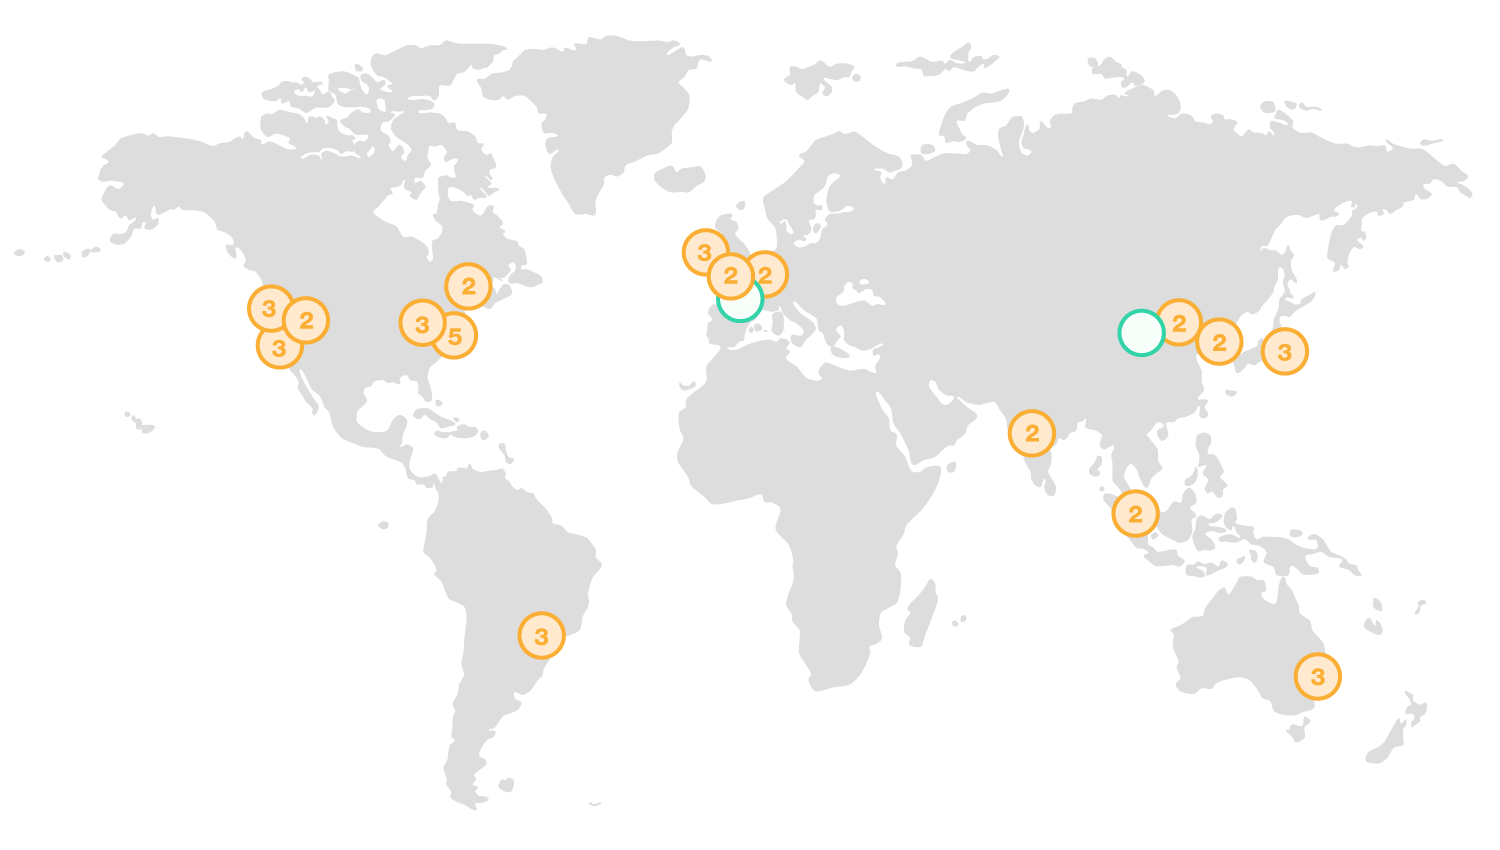
\includegraphics[width=0.9\textwidth]{images/regions.png}
  \caption{weltweite Infrastruktur (orange: Region mit x AZs, weiß/grün: geplante Region) \cite{aws:regions}}
\end{figure}

Eine Region entspricht einem physischen Ort auf der Welt, welcher mehrere Availability Zones (AZs) beherbergen kann. Bei einer AZ handelt es sich um ein oder mehrere unabhängige Rechenzentren, wobei jedes eine redundante Energieversorung, Netzwerk und Konnektivität besitzt.

\begin{figure}[!ht]
  \centering
  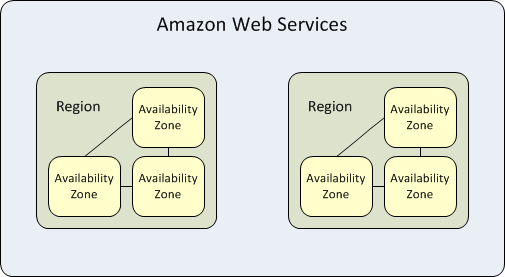
\includegraphics[width=0.7\textwidth]{images/azs_regions.png}
  \caption{Regionen mit zugehörigen Availability Zones \cite{aws:azs}}\label{figure:azs-regions}
\end{figure}

Dies erhöht die Ausfallsicherheit im Falle physischer Schäden z.B. Stürme und ist ein Alleinstellungsmerkmal gegenüber fast allen anderen Anbietern für technologische Infrastrukturen. Es ist daneben auch möglich, Daten zwischen mehreren AZs auszutauschen, um dem Ausfall der Anwendung bei einem Ausfall von AZs in einer Region vorzubeugen. Die AZs sind dafür mit schnellen, privaten Glasfasernetzwerken verbunden.
Durch die Replikation der Daten über mehrere geografische Regionen hinweg, kann die Redundanz und Fehlertoleranz noch zusätzlich erhöht werden.

Die weltweit verteilten Datenzentren sind gerade für international agierende Unternehmen interessant. Je näher ein Datenzentrum dem Endkunden einer Anwendung ist, welche bei AWS gehostet wird, desto geringer fallen die Latenzzeiten aus. Darüberhinaus punktet Amazon mit diesem Konzept beim Thema Datenschutz. In Frankfurt am Main sind 2014 zwei AZs entstanden um Bedenken deutscher Unternehmen hinsichtlich Datenschutz auszuräumen. Kunden können definieren, dass ihre Daten ausschließlich in deutschen Rechenzentren gehalten und bearbeitet werden. Damit unterliegen die dort gehosteten Daten den deutschen Datenschutz-Vorgaben.

Aktuell sind fünf weitere Availability Zones und zwei weitere Regionen geplant.
\\ \cite{computerwoche:reder}, \cite{aws:regions}, \cite{aws:azs}


\section{Vorteile}
\label{sec:vorteile}
Warum ein Einsatz der Amazon Web Services für Unternehmen jeder Größe sinnvoll sein kann, zeigen die Vorteile:
\begin{enumerate}
  \item Kostenersparnis
  \\ An oberster Stelle der Vorteile eines Einsatzes von IT-Ressourcen in der Cloud gegenüber einem klassischen Rechenzentrum stehen die Kosten. Statt einer Aufstellung der IT-Ressourcen für die nächsten Jahre, können Ressourcen bei AWS nach Bedarf beansprucht werden. Ist die Zugriffsrate auf die Webseite gerade sehr hoch, können in wenigen Minuten weitere Server bereitgestellt werden, um die Gesamtlast aufzuteilen. Bezahlt wird dabei nach dem "`Pay-per-use"'-Prinzip. Es werden nur Kosten für Ressourcen erhoben, die auch tatsächlich verwendet wurden.
  \item Hohe Innovations-Geschwindigkeit
  \\ Im Jahr 2015 hat Amazon 722 neue Services und Features umgesetzt. 40\% mehr als im Jahr zuvor. Wöchentlich werden neue Features und Verbesserungen veröffentlicht. Möglich wird das durch viele kleine Teams, die unabhängig voneinander arbeiten. Dabei stehen die Umsetzung der Wünsche der mittlerweile über eine Millionen Kunden im Vordergrund.
  \item Weltweite Infrastruktur
  \\ AWS Nutzer können auf ein Netzwerk weltweit verteilter Datenzentren zurückgreifen. Siehe Sektion \ref{sec:regions}
  \item Arbeitserleichterung
  \\ Auf Wunsch übernimmt AWS mit seinem enormen Dienstangebot notwendige Arbeiten der Nutzer, die sie sonst in Eigenregie erledigen bzw. verwalten müssten. Zum Beispiel Load Balancing zwischen den Servern oder das Aufsetzen eines E-Mail-Service.
  \item Automatisierung
  \\ Viele Dinge, die einen gewissen manuellen Aufwand und ab einer gewissen Komplexität auch eine kognitive Herausforderung bedeuten, können über Skripte automatisiert werden. Via Code können Instanzen aufgesetzt oder Container und Datenbanken bereitgestellt werden. Um Abhängigkeiten muss sich der Anwender dabei nicht sorgen, denn das übernimmt der Computer ganz automatisch. Die Infrastruktur kann beliebig flexibel definiert werden ohne dass manuelle Einstellungen auf der AWS Webseite getätigt werden müssen. Und das Beste daran ist, dass diese Skripte über ein Versionierungs-Tool versioniert werden können und im Fall eines Komplettabsturzes des Systems selbiges in sehr kurzer Zeit neu aufgesetzt werden kann. {\color{red}Vergleich Infrastructure as Code}
  \item Skalierbarkeit
  \\ Neben den Kosten ist Skalierbarkeit wohl das stärkste Argument für eine IT-Infrastruktur in der Cloud. Im Gegensatz zur "`klassischen"' IT, bei der weit in die Zukunft geplant werden und zukünftige Zugriffszahlen abgeschätzt werden mussten, können bei AWS Ressourcen innerhalb von Minuten hinzugeschaltet werden. Sollte der Ansturm vorbei sein und Ressourcen nicht mehr benötigt werden, können diese ebenso schnell wieder abgeschaltet werden, Das ist agil, umweltfreundlich und spart auch noch Geld. Nicht nur zum Auffangen schwankender Zugriffszahlen, auch für das schnelle Bereitstellen von Testsystemen stellt eine hohe Skalierbarkeit der IT-Ressourcen einen großen (Geschwindigkeits-)Vorteil dar.
  \item Ausfallsicherheit
  \\ Die meisten angebotenen Dienste implizieren bereits eine Ausfallsicherheit, so dass sich der Anwender um dieses Problem auch nicht mehr kümmern muss.
  \item Schnelle Anpassungsfähigkeit
  \\ Durch die bereits erwähnte hohe Skalierbarkeit ist auch eine flinke Anpassung an sich ändernde Anforderungen z.B. durch den sich schnell wandelnden Markt gegeben. Entwicklungszyklen können deutlich kürzer ausfallen, da Testsysteme schneller bereitgestellt und Tests schneller durchgeführt werden können.
  \item Die Menge macht's
  \\ Je mehr Kunden AWS nutzen, desto günstiger werden die Dienste für den Einzelnen. Denn um die stetig wachsende Nutzerzahl mit gleichbleibendem Service bedienen zu können, müssen die unterliegenden Prozesse so optimal wie möglich sein.
  \begin{figure}[!ht]
    \centering
    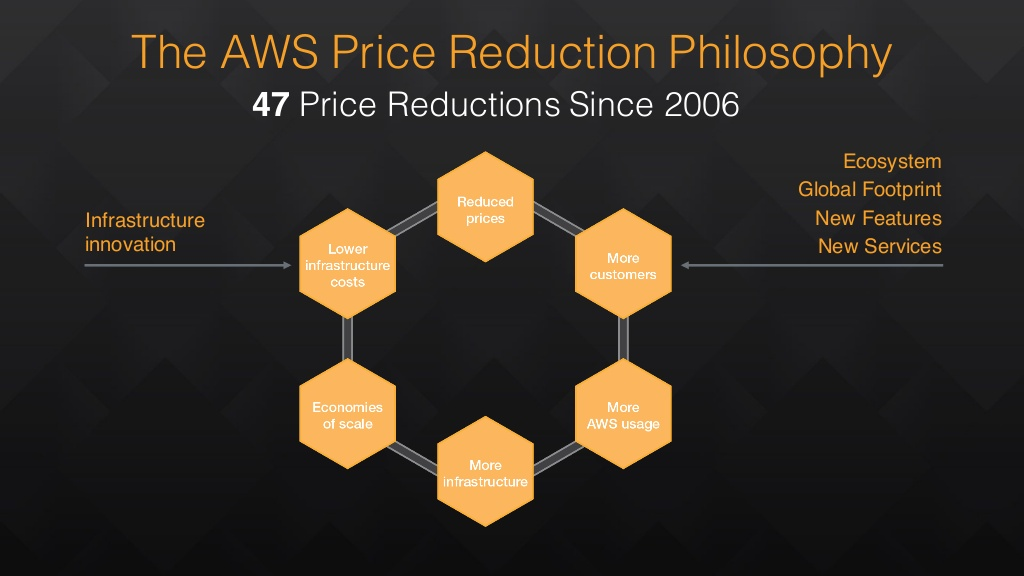
\includegraphics[width=0.9\textwidth]{images/price-reduction.jpg}
    \caption{Preis-Reduktions-Philosophy \cite{aws:insider}}
  \end{figure}
  \item Professionalität
  \\ AWS setzt verschiedene Standards ein, um z.B. Zahlungssicherheit und Datensicherheit zu gewährleisten. Für weitere Informationen zu eingesetzten Standards siehe Kapitel 1.3.9 \cite{wittig:awsinaction})
\end{enumerate} \cite{aws:insider}, \cite{wittig:awsinaction}, \cite{vliet:programmingec2}


\section{Kosten}
Die Kosten für AWS sind abhängig von der Nutzung ("`pay-per-use"'-Prinzip). Zum Beispiel wie viel Speicherplatz verbraucht wird oder wie viel die Laufzeit eines virtuellen Servers beträgt. Dieses Konzept ist gerade für kleine Unternehmen mit einem geringen Budget interessant, da sie weitaus bessere Möglichkeiten haben von Beginn an fehlertolerante Systeme aufzusetzen. Der Betrieb eines großen Servers kostet am Monatsende ebenso viel wie der Betrieb zweier kleinerer Server mit der selben Kapazität wie der große Server. Jedoch bietet die Infrastruktur mit zwei Servern die Möglichkeit redundanter Datenhaltung.
\\Für zukünftig geplante Installationen bietet AWS auf seiner Seite einen Preisrechner \cite{aws:calc}.
\\ Seit 2010 bietet Amazon die Möglichkeit, in begrenztem Maße beliebte Dienste und Rechenleistung (750 Stunden) für 12 Monate kostenlos auszuprobieren. Dieses Programm nennt sich "`Free Usage Tier"'. \cite{wikipedia:aws}, \cite{wittig:awsinaction}

\section{Sicherheit}
Die Sicherheit der eigenen gehosteten Daten ist einer der wichtigsten Punkte, die Amazon gewährleisten muss. Um deutschen Datenschutz- und Datensicherheitsstandards gerecht werden zu können, wurden zwei Datenzentren in Frankfurt am Main eröffnet. Die Daten werden auf Wunsch der Kunden nicht auf amerikanischen Servern gespiegelt und es steht Entwicklern ausdrücklich frei, die hinterlegten Daten zu verschlüsseln. Allerdings war in der Vergangenheit auch immer wieder von Sicherheitslücken die Rede und auch die Auftragsvergabe einer public cloud der CIA an Amazon wurde hinsichtlich des Datenschutzes kritisch beurteilt \cite{computerwoche:sicherheit}, \cite{sueddt:cia}.

% keep an blank line above

\newpage\chapter{AWS am Beispiel einer Sharing Energy Plattform}\label{chapter:kapitellabel} %%%%%%%%%%%%%%%%%%%%%%%%%%%%
Nachfolgend möchte ich anhand eines Beispiels aus dem Energiemarkt einige Dienste von AWS näher betrachten und ihre Wirkungsweise im Zusammenhang darstellen.

\section{Das Fallbeispiel}
\label{sec:fallbeispiel}
Bei LichtBlick, Deutschlands größtem unabhängigen Ökostromanbieter, arbeitet aktuell ein Team an einer neuen Plattform-Idee. Grundsätzlich soll es möglich sein, dass sich Personen gegenseitig ihren selbst erzeugten Ökostrom verkaufen, ohne dass ein Stromhändler dazwischen hängt. Ähnliche Produkte gibt es bereits auf dem niederländischen und dem australischen Markt, jedoch noch nicht in Deutschland. Grund hierfür sind diverse Regularien, die es Besitzern von Wind-, Wasserkraft-, Photovoltaik- und Kraft-Wärme-Kopplungs-Anlagen erschweren, ihren Strom direkt zum Verkauf an andere Personen anzubieten. Da die Entwicklung in diesem Bereich noch recht unklar ist, dennoch erste Ideen auf dem deutschen Markt vertestet werden wollen, entscheidet sich das Team für eine agile und schlanke Herangehensweise. Daher fiel die Wahl bei der Frage nach der erforderlichen IT-Infrastruktur auf Amazon Web Services.

\pagebreak
\section{IT-Infrastruktur}
\label{sec:infrastruktur}

\begin{figure}[!ht]
  \centering
  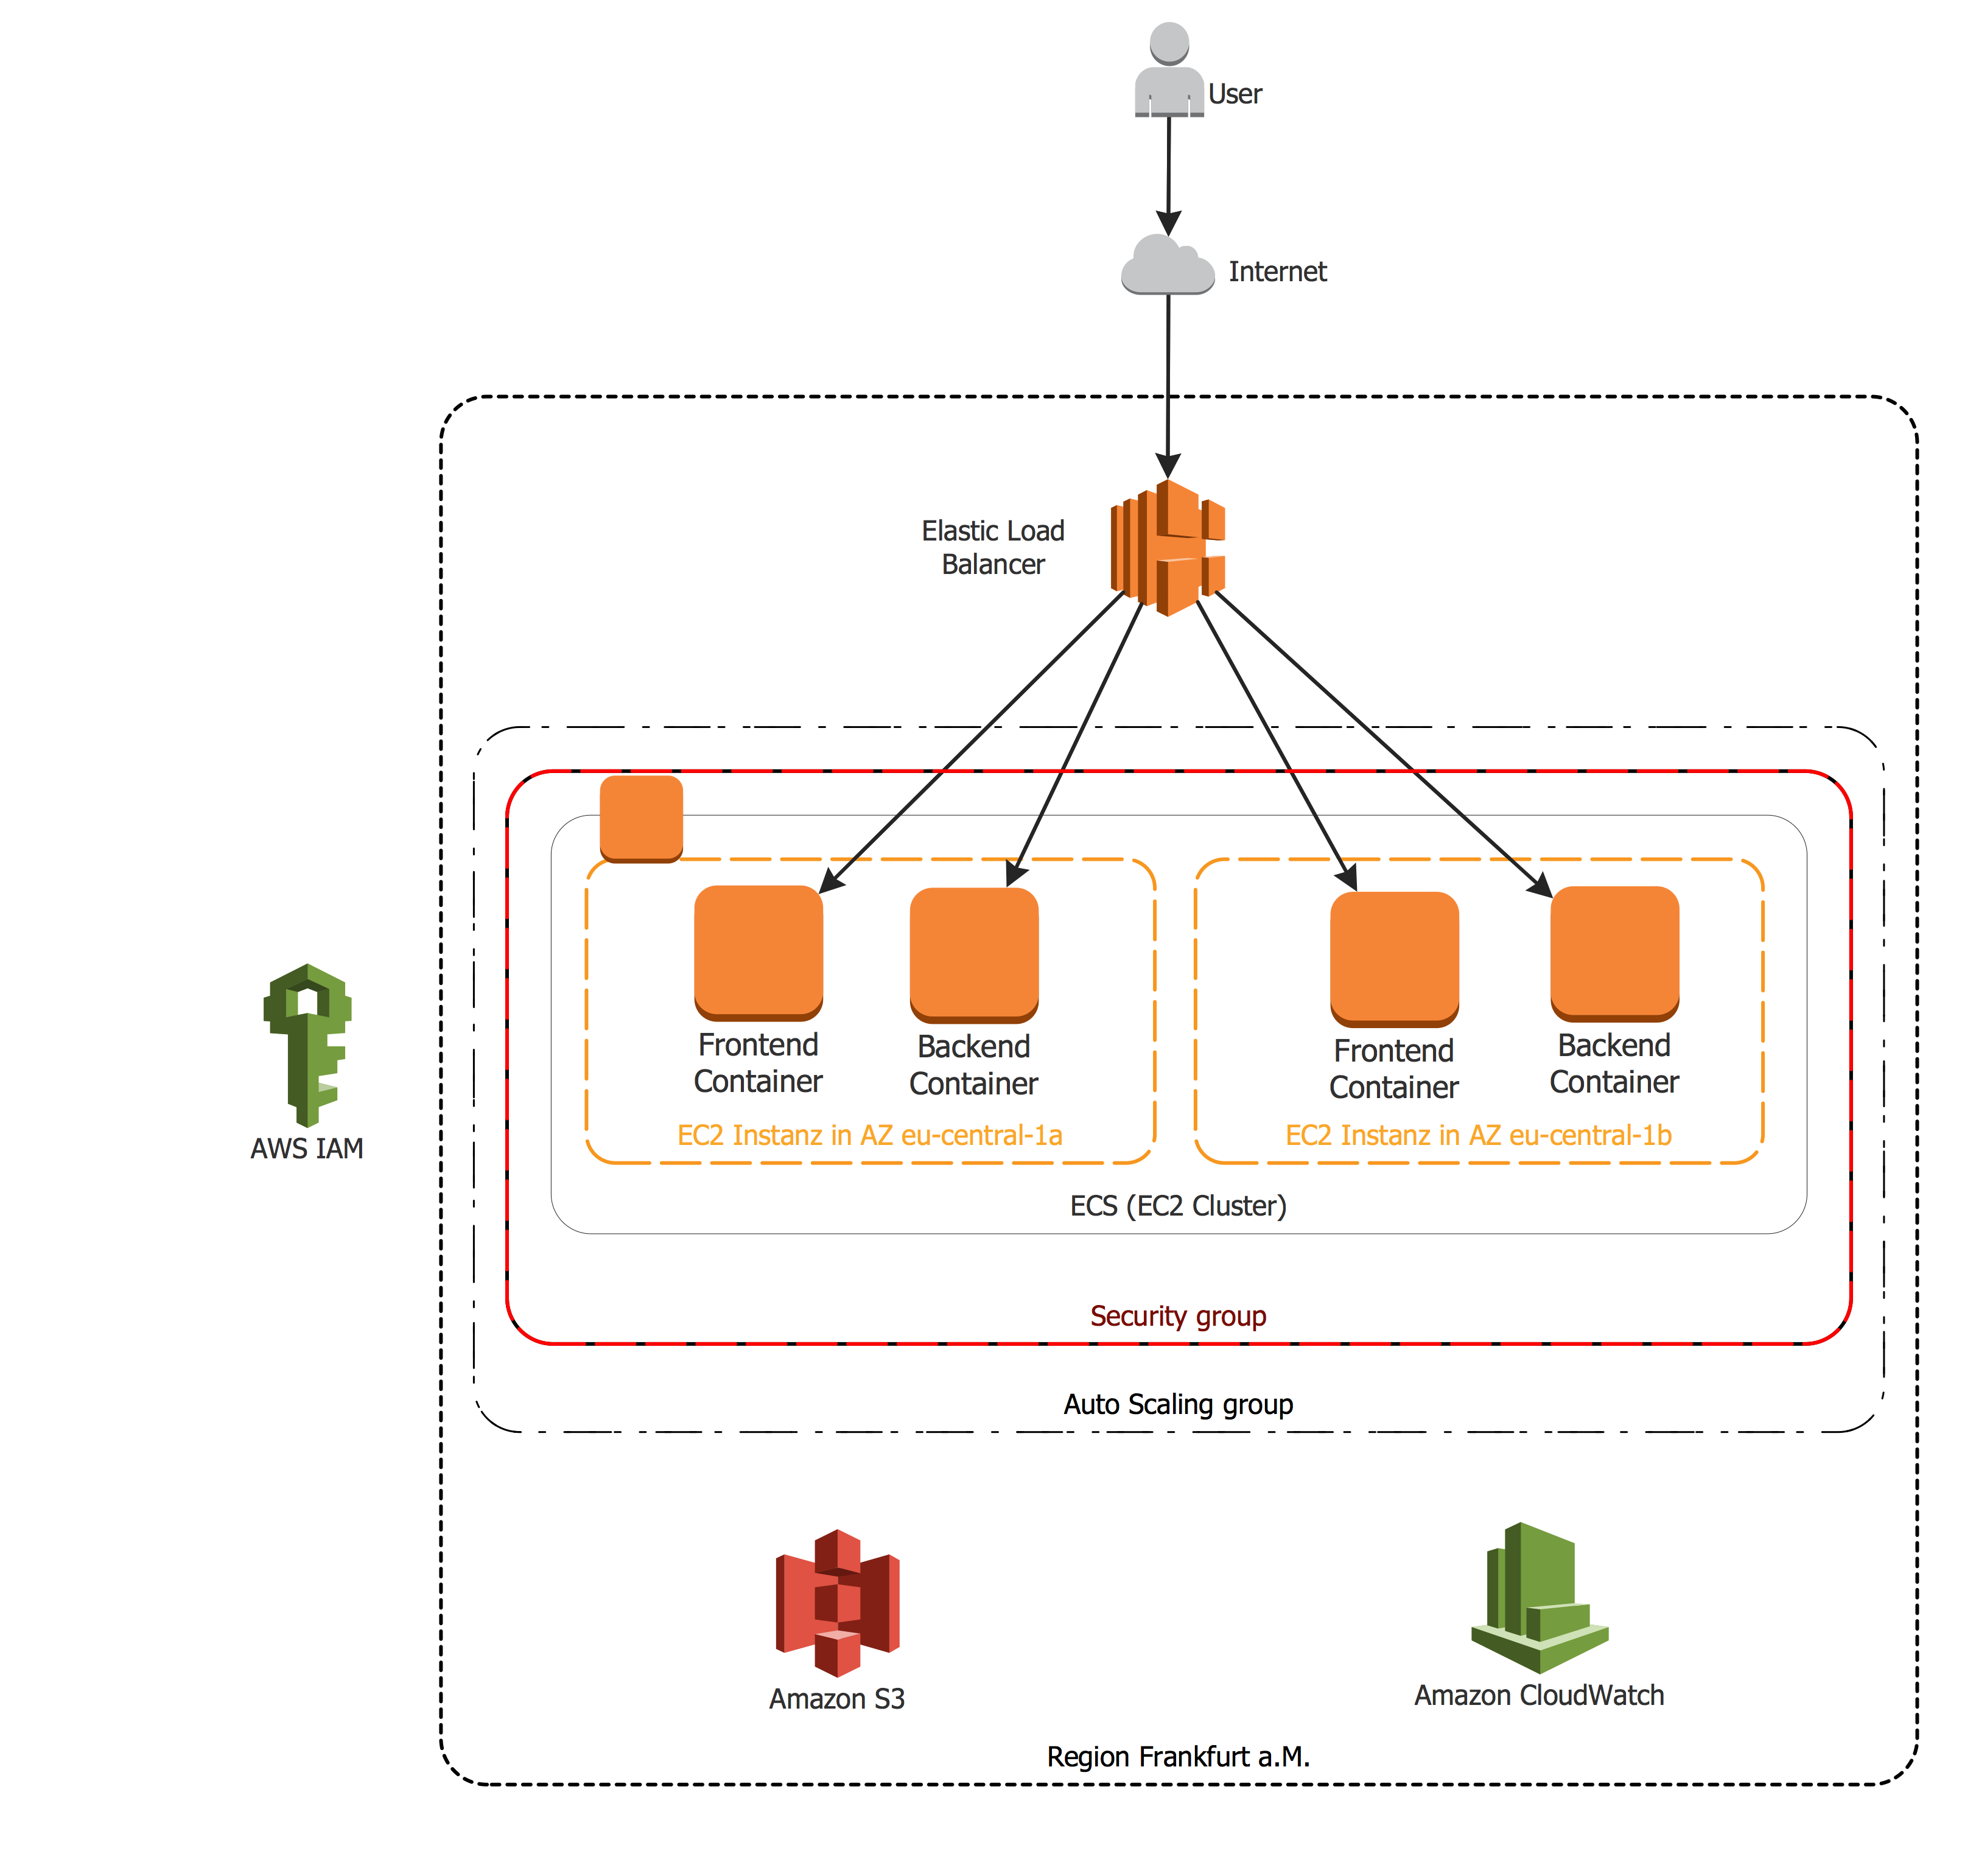
\includegraphics[width=1.0\textwidth]{images/peero.png}
  \caption{Infrastruktur für Sharing Energy Plattform }
\end{figure}

\section{Virtuelle Server mit Elastic Compute Cloud}
\label{sec:ec2}
Jede Anwendung im Web benötigt einen Server, auf dem sie ausgeführt werden kann. Der Webservice Elastic Compute Cloud (EC2) bietet virtuelle Server und damit Rechenleistung in der Cloud, welche je nach Bedarf anpassbar sind. \cite{aws:ec2}
Der Entwickler hat die Möglichkeit, Instanzen von Servern innerhalb weniger Minuten aufzusetzen. Dabei kann er wählen, auf welchem Betriebssystem die Instanz basieren (Windows oder Linux) und welche Ressourcenkonfiguration die bereitgestellte Instanz haben soll. \cite{aws:ec2} \\

Eine Instanz wird aus einem Amazon Machine Image (AMI) erzeugt, welches das Betriebssystem und die darauf installierte Software vorgibt. Amazon bietet verschiedene vorkonfigurierte Images basierend auf 64-bit Windows oder verschiedenen 64-bit UNIX-Derivaten. Dem Nutzer stehen jedoch auch Images von Drittanbietern wie IBM oder Oracle zur Verfügung. Darüberhinaus besteht die Möglichkeit, sein eigenes Image zu entwickeln. Einzige Bedingung ist, dass es auf XEN Hypervisor\footnote{https://www.xenproject.org/} ausgeführt werden kann. \cite{baun:cloudcomp}, \cite{vliet:resilience} \\

Die Ressourcenkonfiguration kann sich aufgrund der Leistungsfähigkeit des Prozessors und der Arbeitsspeicher- und Plattengröße unterscheiden. Die Instanzgrößen variieren von einer kleinen Instanz mit 1,7GB Arbeitsspeicher und 1 EC2 Recheneinheit bis hin zu einer High-CPU Extra Large Instanz mit 7GB Arbeitsspeicher und 20 EC2 Recheneinheiten. \cite{vliet:resilience} \\

Darüberhinaus kann der Nutzer entscheiden, innerhalb welcher Availability Zone die Instanz bereitgestellt wird und ob die Instanzen zusätzlich mit Speicherplatz versehen werden sollen. Dabei hat er die Wahl zwischen zwei Varianten.
\begin{enumerate}
  \item S3-gesichert \\
  Diese Instanztypen können nur neugestartet oder gelöscht werden, da sie einem flüchtigen Speicher entsprechen. Das root device ist Teil der Instanz selbst.
  \item EBS-gesichert \\
  Dieser Typ wird bevorzugt ausgewählt, da Instanzen auch gestoppt und gestartet werden können. Dies wird möglich, da sich die root/boot disk auf einem separaten Elastic Block Store Volume (EBS) befindet, welches unabhängig der Instanz besteht.
\end{enumerate}
\cite{vliet:resilience}, \cite{aws:ec2} \\

Die Instanzen werden in einer virtual private cloud (siehe \ref{sec:vpc}) bereitgestellt. Einem logisch isoliertem Netzwerk, welches verschiedene Netzwerk-Sicherheitsmechanismen mitbringt. Zum Beispiel gehört jede Instanz zu einer oder mehreren Security Groups, um sie gegenüber der Außenwelt abzuschirmen. Angesprochen werden die Instanzen über freigegebene Ports oder IP-Masken. \\
Weiterhin erhalten Instanzen eine öffentliche IP, die sich jedoch mit jeder Bereitstellung der Instanz (z.B. Neustart) ändert. Daher bietet Amazon die Möglichkeit, die öffentliche IPv4-Adresse\footnote{IPv6-Adressen werden derzeit nicht unterstützt} durch eine Elastic IP Adresse auszutauschen. Elastic IP bietet den Vorteil, dass sie konstant bestehen bleibt. Sollte eine Instanz ausfallen, kann die Elastic IP Adresse sehr schnell einer gesunden Instanz zugewiesen werden.
\cite{vliet:resilience}, \cite{aws:eip} \\

In unserem Beispiel verwenden wir aus Gründen der Ausfallsicherheit zwei EC2-Instanzen (Typ: EBS-gesichert) innerhalb eines Clusters, wobei jede zwei identische Services enthält. Den Backend- und den Frontend-Service (siehe \ref{sec:infrastruktur}). Die CLusterung dient der logischen Gruppierung der Instanzen, um geeignete Zugriffsparameter setzen zu können. \\
Jede Instanz liegt in einer anderen Availability Zone in der Region Frankfurt am Main (eu-central-1) und kann auf 4GB Arbeitsspeicher zurückgreifen (Typ: t2.medium). Unterliegend wird ein Linux Image verwendet. \\
Aufgesetzt werden die Instanzen über die AWS API anhand von vordefinierten Konfigurationen, die über TerraForm\footnote{https://www.terraform.io/intro/}-an AWS gesendet werden. Die hierdurch entstehenden Vorteile wurden in Kapitel \ref{sec:vorteile} behandelt. Weitere Möglichkeiten sind
\begin{enumerate}
  \item Amazon Management Konsole
  \item Software Development Kits (SDKs)
  \item Command Line Interface
\end{enumerate} \cite{wittig:awsinaction}

\begin{figure}[!ht]
  \centering
  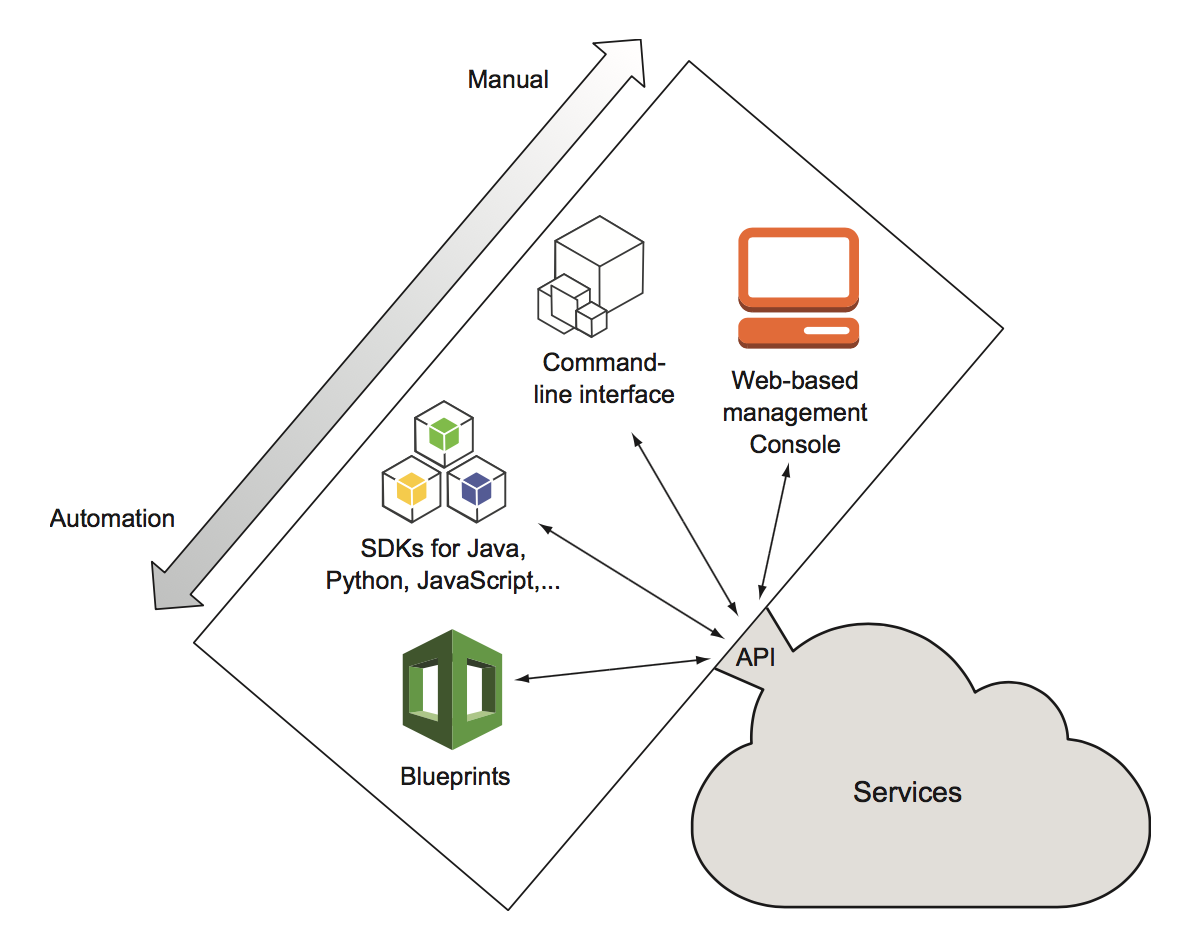
\includegraphics[width=0.7\textwidth]{images/awsapi.png}
  \caption{Interaktionsmöglichkeiten mit der AWS API \cite{wittig:awsinaction}}
\end{figure}

\section{EC2-Container Service}
\label{sec:ecs}
Da unsere Services innerhalb von Docker-Containern laufen, nutzen wir den von Amazon angebotenen EC2-Container Service (ECS). Dieser Dienst wurde speziell für die Unterstützung von Docker-Containern auf EC2-Instanzen entwickelt und erlaubt neben dem Betrieb auch die Verwaltung der Anwendungen auf einem verwalteten EC2-Instanz-Cluster. Der Betrieb einer eigenen Cluster-Managementinfrastruktur entfällt. Funktionen wie Sicherheitsgruppen, Elastic Load Balancing, EBS-Volumes und IAM-Rollen stehen daneben ebenfalls zur Verfügung \cite{aws:ecs}.

\section{Auto-Scaling}
\label{sec:auto-scaling}
Beide Instanzen laufen innerhalb einer Security Group, welche wiederum in einer Auto-Scaling Group liegt. Letztere ermöglicht eine elastische Instanzgruppe, deren bereitgestellte Ressourcen sich je nach Bedarf anpassen. Das Auto-Scaling basiert dabei auf CloudWatch-Metriken wie z.B. CPU-Auslastung. Beispielsweise könnte eine Metrik besagen, dass zwei neue Instanzen gestartet werden sollen, wenn die CPU Auslastung für 5 Minuten bei 60\% oder höher liegt. CloudWatch ist ein Service, der verschiedene Informationen der verwendeten IT-Ressourcen überwacht und misst. Von der Betrachtung einzelner Instanzen bis hin zur Überwachung aller Instanzen einer Region ist nahezu alles möglich. Es ist jedoch auch denkbar, dass die Ressourcenanpassung der Gruppe auf Amazons verteilten Queue-System SQS basiert. Dann würden sich die Ressourcen nach der Anzahl der Items in der Queue richten. \cite{vliet:resilience}, \cite{vliet:programmingec2} \\

In unserem Projekt haben wir noch keine konkreten Metriken definiert, die für das AutoScaling herangezogen werden sollen. Allerdings würden wir uns vermutlich im ersten Schritt auf die CPU-Auslastung stützen.

\section{Load Balancing}
\label{sec:elb}
Der gesamten Gruppe vorgesetzt ist ein Application Load Balancer (ALB), der die Instanzen vom öffentlichen Internet loslöst. Ein ALB ist eine von zwei Lastenverteilungsoptionen\footnote{neben Classic Load Balancer; \\vgl. Funktionen https://aws.amazon.com/de/elasticloadbalancing/classicloadbalancer/faqs/} des Services Elastic Load Balancing.
Der Elastic Load Balancer (ELB) sitzt vor einer Gruppe von EC2-Instanzen und kann jede Art von TCP Traffic verteilen. Bei der Kommunikation mit den Instanzen nutzt der ELB HTTP und wandelt ggf. vorher eingegangenes HTTPS in HTTP um. Dieses Vorgehen reduziert die Belastung der Instanzen und erhöht damit die Fehlertoleranz. Bei der Verteilung des Traffics achtet der ELB auf eine gleichmäßige Verteilung auf alle Availability Zonen und in jeder AZ auf die gleichmäßige Aufteilung auf die vorhandenen Instanzen. Dies eröht die Sicherheit und reduziert die Komplexität der Infrastruktur. \\
Wird der ELB zusammen mit einer Auto-Scaling Group betrieben, kann dieser je nach Bedarf automatisch Instanzen registrieren und bei Nicht-Gebrauch auch wieder abmelden. Eine manuelle Zuordnung der IPs zu den jeweiligen Instanzen ist damit nicht mehr nötig. Bei der Abmeldung einer bestehenden Instanz und nachfolgender Neu-Registrierung einer neuen Instanz kann es unter Umständen kurzzeitig dazu kommen, dass der Dienst nicht zur Verfügung steht. Dieses Problem ist bekannt und entsteht dadurch, dass die alte Instanz erst beendet wird, ehe die neue Instanz hochgefahren werden kann.
Dem ELB kann ein Hostname zugeordnet werden, worüber dieser direkt angesprochen werden kann.
\cite{vliet:resilience}, \cite{aws:elb} \\

\subsection{Application Load Balancer}
\label{sec:alb}
Bei dem zuvor erwähnten ALB, welchen wir im Einsatz haben, verteilt sich der eingehende Traffic auf erweiterte Anwendungsinformationen, die die Inhalte der Anfrage enthalten. Damit eignet sich dieser Typ besonders für Anwendungen mit der Notwendigkeit erweiterter Routing-Funktionen, Micro-Services und Container-basierten Architekturen. Ein ALB ermöglicht die Lastenverteilung auf mehrere Ports einer EC2-Instanz, aber auch die Umleitung auf mehrere Services. Letzteres wird durch Target Groups (siehe \ref{sec:target-group}) und inhaltsbasiertes Routing ermöglicht, welches Anfragen basierend auf ihrem Inhalt an den entsprechenden Service weiterleitet.\footnote{weitere Funktionen des ALBs können \cite{aws:alb} entnommen werden} \cite{aws:elb}, \cite{aws:alb}

\begin{figure}[!ht]
  \centering
  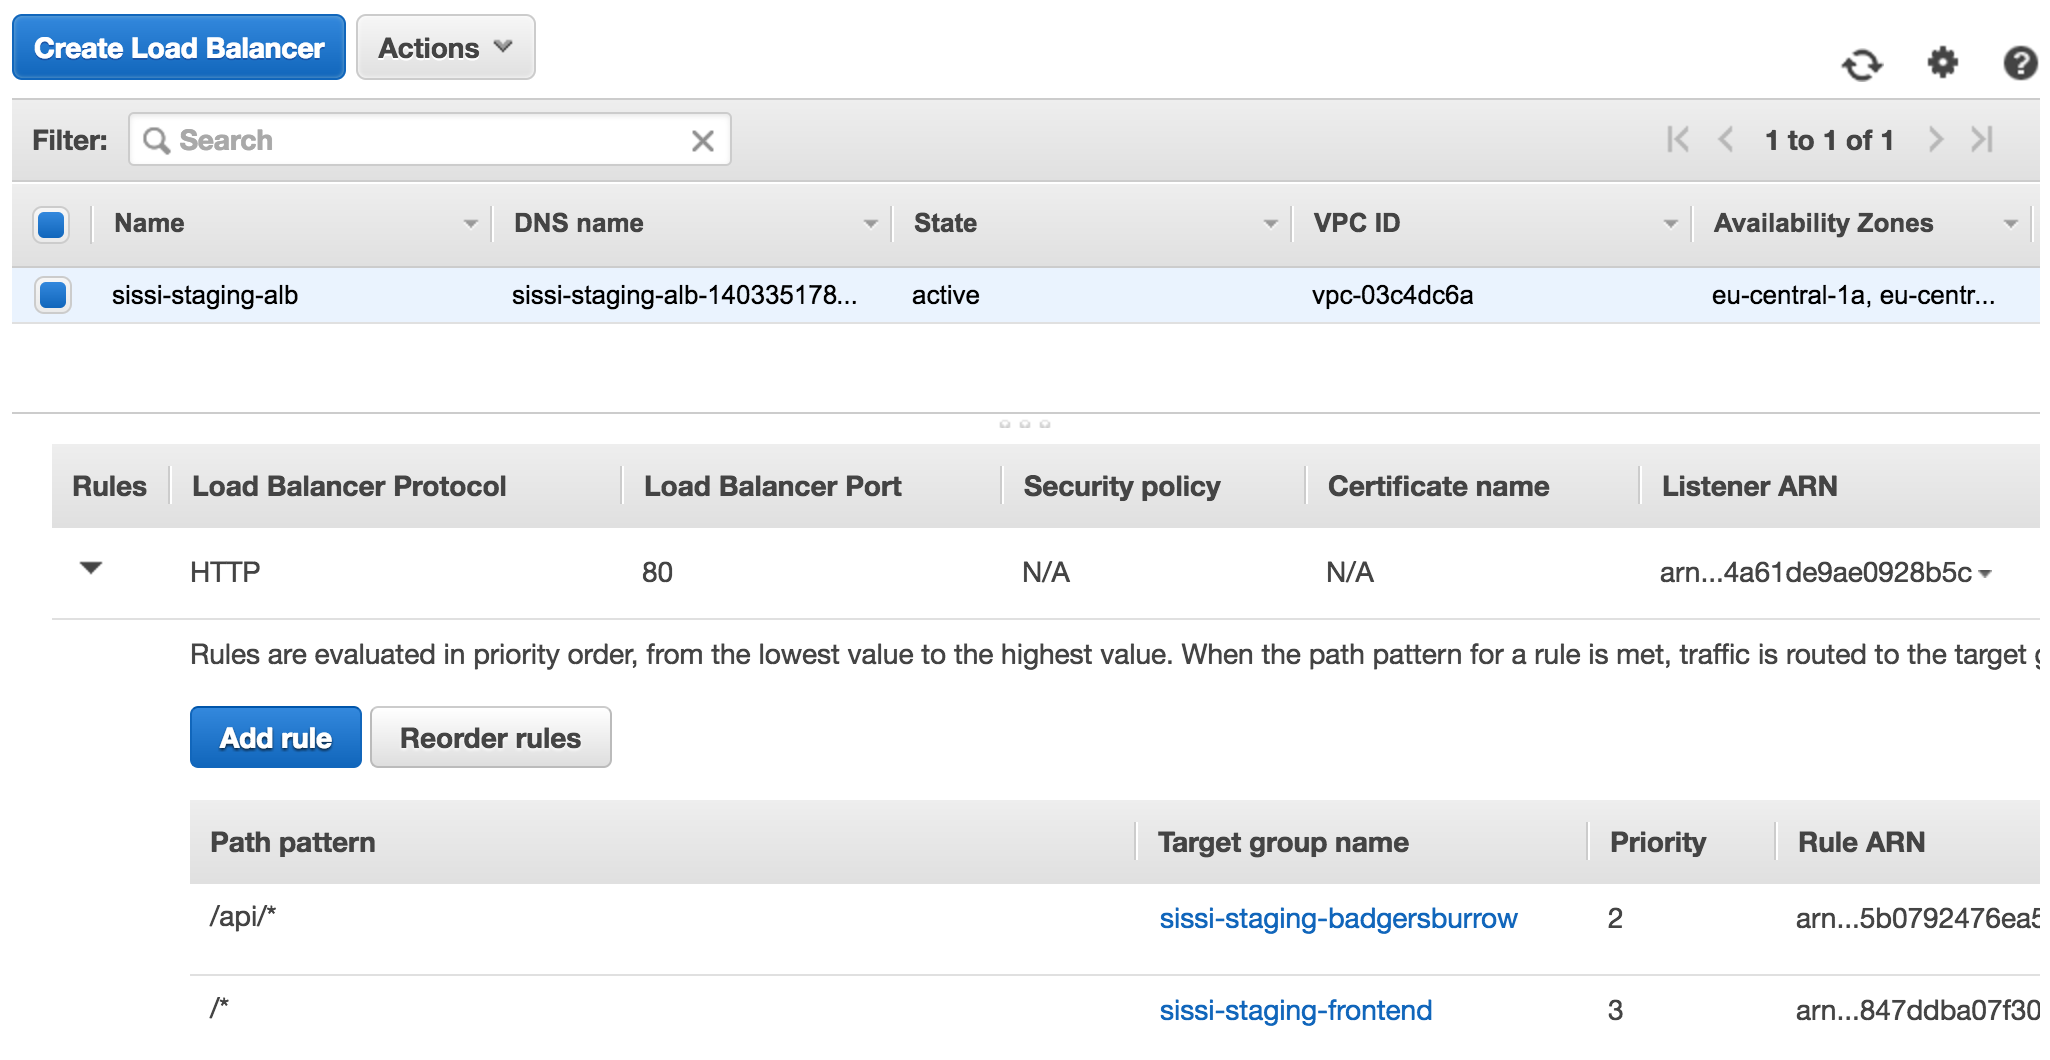
\includegraphics[width=0.9\textwidth]{images/routing.png}
  \caption{Screenshot aus AWS-Entwicklerkonsole mit Listener-Regeln des ALB für inhaltsbasiertes Routing}
\end{figure}

\subsection{Target-Group}
\label{sec:target-group}
Eine Target Group ist eine Gruppierung von Instanzen oder Microservices innerhalb der Instanzen, damit Anfragen durch den ALB (siehe \ref{sec:alb}) gezielt an den zuständigen Dienst geroutet werden können. Hierfür wird eine Target Group als eine Regel für einen Listener des Load Balancers definiert. Jede Target Group nutzt die Standard Health Check- Einstellungen eines Load Balancers. Auf Basis dessen kann der Load Balancer ausschließlich gesunde Targets ansprechen. \cite{aws:target} \\

In unserem Fallbeispiel gibt es zwei Target Groups. In beiden befinden sich beide verfügbaren Instanzen als Targets. Wie bereits in Kapitel \ref{sec:ec2} beschrieben, befinden sich in jeder Instanz jeweils zwei Services, weshalb die eigentliche Logik der Target Groups bei uns (noch) nicht korrekt greift. Richtiger wäre eine Target Group für alle Backend-Services und eine Target Group für alle Frontend-Services. Je nach Auslastung würde dann der eine über den anderen Service innerhalb der Target Group bevorzugt angesprochen. Unser Aufbau ist derzeit noch der Tatsache geschuldet, dass wir lediglich zwei Instanzen innerhalb unseres Clusters haben und der Scheduler die Container für einen Service bestmöglich gleichmäßig darauf verteilt.


\section{Virtual Private Cloud}
\label{sec:vpc}
Der im vorherigen Kapitel erwähnte ALB ist der einzige Kontakt zur Außenwelt. Dies dient zum einen der Sicherheit und zum anderen dem Pragmatismus, da nicht für jeden einzelnen virtuellen Server ein DNS Name vergeben und verwaltet werden muss. Der ALB bekommt einen eindeutigen Hostnamen, über den der ALB und damit alle dahinterliegenden Services innerhalb der definierten Security Groups erreichbar sind. Die Security Groups bieten jedoch nicht ausreichend Kontrollmöglichkeiten für das sichere Handling der Anfragen. Zum Beispiel ist es in normalen Security Groups nicht möglich, eingehende Anfragen zu beschränken. Um eingehenden und ausgehenden Datenverkehr kontrollieren zu können, bietet Amazon die Virtual Private Cloud (VPC) an. \\
Der Einsatz der VPC ermöglicht es uns, die beiden EC2-Instanzen in einem privaten Sub-Netzwerk unterzubringen. Der ALB befindet sich im öffentlichen Netzwerk, welches von außen sichtbar ist. Anfragen gelangen per HTTPS über den Hostnamen zum ALB, wo sie umgewandelt und per HTTP an die jeweiligen Services in den EC2-Instanzen weitergeleitet werden.
\cite{vliet:resilience}, \cite{wittig:awsinaction}, \cite{aws:vpc}

\section{Simple Storage Service}
\label{sec:s3}
Zur dauerhaften Speicherung erhobener Daten der Nutzer verwenden wir den neben EC2 zweiten Basisdienst für Webanwendungen: Amazons Simple Storage Service (S3). Ein virtueller Objekt-Speicher zur Speicherung einer unbegrenzten Datenmenge. Amazon proklamiert eine 99,999999999\% Haltbarkeit und 99,99\% Verfügbarkeit der Daten. Es soll nahezu unmöglich sein, dass Dateien kaputt oder verloren gehen. Amazons Chief Evangelist Jeff Barr beschreibt es so \\
\begin{quote}
"`If you store 10.000 objects with us, on average we may lose one of them every 10 million years or so."'
\end{quote} \cite{vliet:programmingec2}

Sichergestellt wird dies über ein Service Level Agreement. \cite{vliet:programmingec2}

Zu speichernde Objekte werden in buckets vorgehalten. Diese können in jeder Region erstellt werden und eine unbegrenzte Anzahl Objekte mit Größen zwischen 1Byte und 5TB enthalten. Zur Speicherung statischer Informationen von Webseiten oder mobilen Anwendungen ist S3 weniger geeignet. Hierfür kann der Nutzer auf CloudFront ausweichen. einem Content Distribution Network, das dem Verteilen statischer, dynamischer und gestreamter Inhalte über die gesamte Welt dient.
\cite{vliet:resilience}, \cite{aws:s3}

\section{Identity Access Management}
\label{sec:iam}
Zur Einschränkung der Zugriffsmöglichkeiten für Nutzer auf die IT-Ressourcen in AWS und damit zur Erhöhung der Sicherheit, bietet AWS den Identity and Access Management Service (IAM). Dieser Service prüft jede Anfrage auf deren Zulässigkeit. Zugriffe können über policies Benutzer- oder Gruppenscharf organisiert werden. Die Authentifizierung der Nutzer gegenüber der Services erfolgt über die Anmeldedaten der Benutzer. IAM bietet neben der Zugriffsverwaltung auch
\begin{itemize}
  \item Multi Factor Authentication (MFA) als zweiten Authentifizierungsschritt für bestimmte Operationen
  \item das Hinzufügen von Rollen zu EC2 Instanzen, wodurch die Festlegungen für die Rolle die Zugriffsmöglichkeiten auf die Instanz bestimmen
\end{itemize}
\cite{vliet:resilience}, \cite{wittig:awsinaction}

% keep an blank line above

\finish
